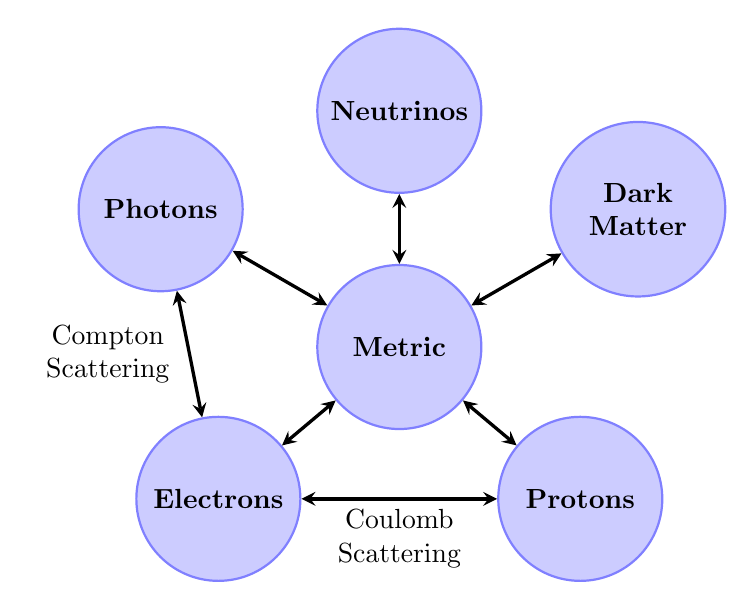
\begin{tikzpicture}[%
    writing/.style={%
      text width=18mm,  % default text width
      align=center      % align in center
    },
    component/.style={%
      circle,           % circular node
      fill=blue!20,     % fill it in blue
      draw=blue!50,     % outside edge in blue
      thick,            %              and thick
      writing,          % writing style above
      font=\bfseries    % bold writing
    },
    connection/.style={%
      <->,             % Double headed
      very thick,      % very thick arrows
      >=stealth        % pretty arrow head
    }
]

    % nodes
    \node at (0,0)     [component] (metric)      {Metric};

    \node at (90 :3)   [component] (neutrinos)   {Neutrinos};
    \node at (150:3.5) [component] (photons)     {Photons};
    \node at (220:3)   [component] (electrons)   {Electrons};    
    \node at (320:3)   [component] (protons)     {Protons};      
    \node at (30 :3.5) [component] (dark matter) {Dark Matter};


    % connections
    \draw[connection] (metric) -- (neutrinos);
    \draw[connection] (metric) -- (photons);
    \draw[connection] (metric) -- (electrons);
    \draw[connection] (metric) -- (protons);
    \draw[connection] (metric) -- (dark matter);

    % interconnections with text
    \draw[connection] 
    (electrons) to 
    node[below,writing] {Coulomb Scattering} 
    (protons);

    \draw[connection] 
    (electrons) to 
    node[left,writing] {Compton Scattering} 
    (photons);

\end{tikzpicture}
